%          spconf.sty  - ICASSP/ICIP LaTeX style file, and
        %  IEEEbib.bst - IEEE bibliography style file.
% --------------------------------------------------------------------------
\documentclass{article}
\usepackage{spconf,amsmath,amssymb,graphicx}
\usepackage{booktabs}
\usepackage{hyperref}
\usepackage{float}          % 支持浮动体
\usepackage{algorithm}
\usepackage{algorithmic}



% Title.
% ------
\title{Bridging the Data Gap: Leveraging AI to Address Data Scarcity in Medical Imaging}
\name{SN: 24076607}
\address{}
%
\begin{document}

%
\maketitle
%
\begin{abstract}
    This section provides a brief overview of the methodology/results presented in the report.\footnote{The Blog is provided \url{https://yushiran.github.io/ELEC0139_BLOG_SN24076607/} and GitHub project: \url{https://github.com/yushiran/ELEC0139_BLOG_SN24076607}}
\end{abstract}
%
\begin{keywords}
    One, two, three, four, five
\end{keywords}
%

\section{Application Domain and Challenges}
\label{sec:app_domain}

\subsection{The Application Domain: Medical Imaging}
Medical imaging is pivotal in modern diagnostics, providing non-invasive methods to visualize internal structures of the human body. It encompasses a wide range of imaging modalities, including magnetic resonance imaging (MRI), computed tomography (CT), and X-rays, each offering different contrast mechanisms and spatial resolutions to support clinical diagnosis and treatment planning.

In recent years, medical imaging has been revolutionized by the advances in computer vision and deep learning technologies​\cite{upadhyayAdvancesDeepLearning2024}. 
These technologies have significantly enhanced the capability of automatic image analysis systems, particularly in tasks like medical image segmentation (MedSeg), which involves partitioning images into regions corresponding to specific organs or lesions such as the chest, brain, abdomen, eye, and heart\cite{sushankiReviewComputationalMethods2024}​.

Among the imaging modalities, CT scans, MRI, and X-rays are especially critical in detecting and monitoring various health conditions. For instance, CT imaging has been extensively used in diagnosing lung infections during the COVID-19 pandemic, as evidenced by the segmentation of lung infection regions in CT scans​\cite{LIU2020244,9446143,YI2019101552}.

The segmentation process itself plays a fundamental role in medical image analysis by enabling pixel-level identification of anatomical structures, facilitating precise diagnosis and personalized treatment​\cite{kumarTripleClippedHistogramBased2021}. Manual segmentation by radiologists, although accurate, is labor-intensive, time-consuming, and costly, thus driving the demand for automated methods that leverage deep learning​\cite{TAJBAKHSH2020101693}.

Overall, medical imaging, supported by modern computational methods, forms the cornerstone of contemporary healthcare, enabling earlier detection, better disease monitoring, and improved patient outcomes.

\subsection{Current Challenges: Data Scarcity and Its Implications}
Medical image segmentation has witnessed tremendous progress with deep learning, yet its success remains heavily dependent on the availability of large-scale, high-quality annotated datasets. Unfortunately, several persistent challenges hinder the widespread deployment of AI models in medical imaging, especially in real-world clinical environments.

\subsubsection{Limited Annotated Datasets}
Obtaining labeled medical imaging data is a labor-intensive and costly process, typically requiring the expertise of trained radiologists and high-end equipment. Manual annotation, such as pixel-wise segmentation, is especially time-consuming. As a result, the availability of large annotated datasets remains limited​. Moreover, privacy regulations and patient confidentiality further restrict data sharing and public availability​\cite{TAJBAKHSH2020101693}.

\subsubsection{Bias and Generalizability Issues}
Even when labeled datasets are available, they are often limited in diversity, both demographically and technically (e.g., variation in scanner models or acquisition protocols). This lack of heterogeneity leads to significant distribution shift problems when models trained on one dataset are deployed on another, ultimately affecting their generalization performance across populations and institutions​.

\subsubsection{Resource Constraints}\
Healthcare systems in low- and middle-income regions face acute shortages in data collection infrastructure and medical imaging resources. The high costs of annotation and hardware requirements for data processing place an additional burden on AI development in such contexts. As noted in the literature, while deep learning architectures like U-Nets are widely adopted in academic research, deploying them in under-resourced settings remains a formidable challenge​.

\subsection{The Case for AI/ML Technologies}
This subsection makes the case for adopting machine learning and artificial intelligence technologies to address the challenges and improve outcomes in the application domain.

\subsubsection{Efficient Data Utilization}
AI techniques, especially deep learning architectures like U-Nets, are capable of learning meaningful spatial and semantic patterns even from limited labeled data. When designed appropriately, such models can achieve strong segmentation performance despite inherent challenges like noise and distribution shift​
\cite{vermaRoleDeepLearning2023}. Moreover, hybrid architectures such as U-Net++ and attention mechanisms have further improved efficiency and robustness​
\cite{zhouUNetNestedUNet2018}.

\subsubsection{Synthetic Data Generation}
Synthetic data generation using generative adversarial networks (GANs) is one of the most promising avenues for alleviating labeled data scarcity. For instance, models like Cycle-GANs and conditional GANs have been used to generate high-fidelity synthetic MRI and ultrasound images that closely resemble real samples, including segmentation labels. These synthetic datasets, when used in model training, have shown comparable performance to real data\cite{9324763,shinMedicalImageSynthesis2018}​.

\subsubsection{Self-Supervised Learning}
Self-supervised learning (SSL) has gained traction in medical image analysis due to its ability to leverage vast amounts of unlabeled data. Techniques such as context restoration, multi-modal feature fusion, and attention-based pseudo labeling enable models to learn robust representations without requiring ground-truth masks​
​\cite{CHAITANYA2021101934,zhengHierarchicalSelfsupervisedLearning2021}.




\section{AI/ML Solutions to Data Scarcity in Medical Imaging}
\label{sec:ml_technologies}

\subsection{Self-Supervised Learning (SSL)}

Self-supervised learning (SSL) enables the use of large amounts of unlabeled data to pretrain neural networks by defining pretext tasks—artificial supervision signals derived from the data itself. In medical imaging, this is particularly valuable, as obtaining labeled data is expensive and requires expert input​.

Chen et al. (2019)\cite{chenSelfsupervisedLearningMedical2019} proposed a context restoration strategy tailored to the characteristics of medical images. The method corrupts the spatial arrangement of an image by swapping randomly selected patches and then trains a convolutional neural network (CNN) to restore the original image. This process forces the network to learn semantic-level image representations, which are transferable to downstream tasks such as classification, localization, and segmentation​.

\subsubsection{Key Features of Context Restoration SSL}
\begin{itemize}
    \item \textbf{Semantic Feature Learning:} The network learns to recognize and correct structural inconsistencies, resulting in rich semantic representations.
    \item \textbf{Transferability:} Features learned through this method can initialize both encoder and decoder parts of downstream CNNs, especially useful for segmentation tasks where full image-to-image mapping is needed​.
    \item \textbf{Simplicity:} The approach is simple to implement, with minimal changes to existing architectures and training pipelines.
\end{itemize}

\subsubsection{Methodology}
Let $\mathcal{X} = \{x_1, x_2, \ldots, x_N\}$ be a set of unlabeled medical images. A corruption function $\mathcal{R}$ generates a disordered image $\tilde{x}_i$:
\[
\tilde{x}_i = \mathcal{R}(x_i)
\]
A CNN model $g(\cdot)$ is then trained to restore the original image:
\[
x_i = g(\tilde{x}_i) \approx f^{-1}(\tilde{x}_i)
\]
The training objective is to minimize the pixel-wise L2 reconstruction loss:
\[
\mathcal{L}_{\text{SSL}} = \left\| x_i - g(\tilde{x}_i) \right\|_2^2
\]

The corruption function $\mathcal{R}$ randomly selects and swaps image patches:

\begin{algorithm}[H]
    \caption{Image Context Disordering}
    \begin{algorithmic}[1]
    \STATE \textbf{Input:} original image $x_i$
    \STATE \textbf{Output:} image with disordered context $\tilde{x}_i$
    \FOR{$t = 1$ to $T$}
      \STATE randomly select patch $p_1 \in x_i$
      \STATE randomly select patch $p_2 \in x_i$
      \IF{$p_1 \cap p_2 = \emptyset$}
        \STATE swap $p_1$ and $p_2$
      \ENDIF
    \ENDFOR
    \end{algorithmic}
\end{algorithm}


The CNN model $g(\cdot)$ has two parts, as shown in Figure \ref{fig:context_restoration_architecture}:

\begin{figure*}[htb]
    \centering
    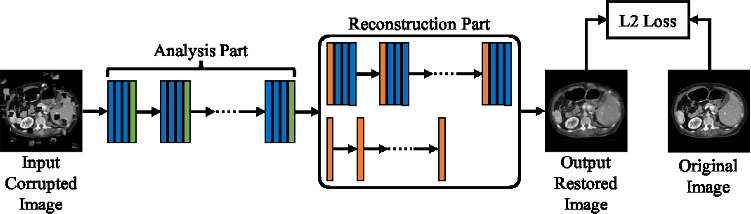
\includegraphics[width=0.98\linewidth]{images/General_CNN_architecture_for_the_context_restoration_self_supervised_learning.pdf}
    \caption{General CNN architecture for context restoration SSL. Blue, green, and orange strides represent convolutional, downsampling, and upsampling units, respectively.}
    \label{fig:context_restoration_architecture}
\end{figure*}

\begin{itemize}
    \item \textbf{Analysis Part:} an encoder that extracts features from the disordered image. It may include convolutional layers, residual blocks~\cite{He2015DeepRL}, or inception modules~\cite{Szegedy2015RethinkingTI}.
    \item \textbf{Reconstruction Part:} a decoder that upsamples the features and reconstructs the image in correct spatial order.
\end{itemize}

\begin{figure}[H]
    \centering
    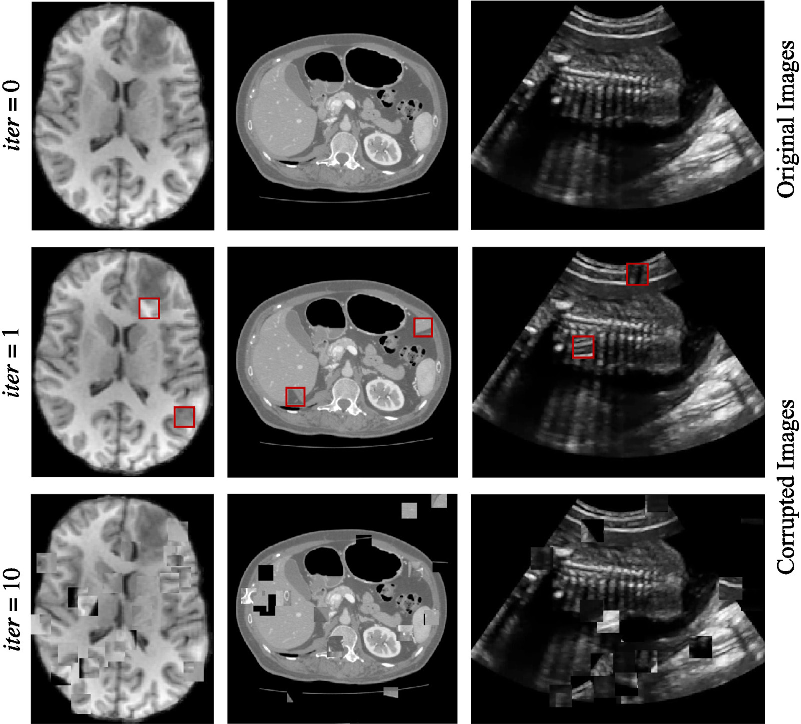
\includegraphics[width=0.98\linewidth]{images/Generating_training_images_for_self_supervised_context_disordering.pdf}
    \caption{Examples of training images for self-supervised context disordering. The second column highlights swapped patches after the first iteration.}
    \label{fig:context_disordering}
\end{figure}



\subsubsection{Applications and Evaluation}
\begin{itemize}
    \item \textbf{Classification:} On fetal ultrasound images, context restoration pretraining improved the F1-score by over 7 percentage points compared to random initialization with only 25\% of training data​.
    \item \textbf{Localization:} For abdominal organ localization in CT images, models initialized via context restoration outperformed those trained with auto-encoders or relative position tasks, especially under data-limited settings​.
    \item \textbf{Segmentation:} In brain tumor segmentation using multi-modal MRI, models with context restoration pretraining achieved higher Dice scores and lower Hausdorff distances than all other SSL and baseline methods​.
\end{itemize}

\subsubsection{Benefits}
\begin{itemize}
    \item Reduces dependence on labeled data by leveraging vast pools of unlabeled medical images.
    \item Improves model performance under limited supervision conditions, particularly in small-sample settings.
    \item Generalizes well across modalities (ultrasound, CT, MRI) and tasks (classification, localization, segmentation).
\end{itemize}

\subsection{Reinforcement Learning (RL)}

Reinforcement Learning (RL) is a powerful machine learning paradigm in which an agent learns to interact with its environment by receiving feedback in the form of rewards. Unlike supervised learning, which relies heavily on large-scale annotated datasets, RL can operate effectively with minimal labeled data, making it particularly attractive in medical imaging domains where data scarcity is a major challenge~\cite{huReinforcementLearningMedical2023}.

An RL framework is typically defined by a set of core components: \textbf{state} (the environment observation), \textbf{action} (possible moves the agent can make), \textbf{reward} (feedback signal guiding learning), and \textbf{policy} (the decision-making strategy). Depending on whether the environment is explicitly modeled, RL approaches are broadly categorized into \textit{model-free} and \textit{model-based} methods. Model-free methods, such as DQN\cite{mnihHumanlevelControlDeep2015a} and A2C\cite{Schulman2017ProximalPO,Mnih2016AsynchronousMF}, learn policies directly through interaction, while model-based approaches attempt to learn a transition model to improve sample efficiency—particularly important in low-data regimes.

\subsubsection{Mathematical Formulation of Reinforcement Learning}

Reinforcement learning problems are often modeled as a Markov Decision Process (MDP), defined by a tuple $\langle \mathcal{S}, \mathcal{A}, \mathcal{P}, \mathcal{R}, \gamma \rangle$, where:
\begin{itemize}
    \item $\mathcal{S}$ is the set of possible states,
    \item $\mathcal{A}$ is the set of actions,
    \item $\mathcal{P}(s' | s, a)$ is the transition probability function,
    \item $\mathcal{R}(s, a)$ is the reward received after taking action $a$ in state $s$,
    \item $\gamma \in [0, 1]$ is the discount factor for future rewards.
\end{itemize}

The goal is to learn a policy $\pi(a|s)$ that maximizes the expected cumulative reward:
\[
J(\pi) = \mathbb{E}_{\pi} \left[ \sum_{t=0}^{\infty} \gamma^t r_t \right]
\]

The value function for a state under policy $\pi$ is:
\[
V^{\pi}(s) = \mathbb{E}_{\pi} \left[ \sum_{t=0}^{\infty} \gamma^t r_t \mid s_0 = s \right]
\]

The action-value function (Q-function) is:
\[
Q^{\pi}(s, a) = \mathbb{E}_{\pi} \left[ \sum_{t=0}^{\infty} \gamma^t r_t \mid s_0 = s, a_0 = a \right]
\]

An optimal policy $\pi^*$ satisfies:
\[
Q^{\pi^*}(s, a) = \max_{\pi} Q^{\pi}(s, a)
\]

This formulation allows reinforcement learning agents to learn optimal decision-making strategies through trial-and-error, without requiring large-scale labeled data. This is especially beneficial in medical imaging applications such as classification, registration, or synthesis, where annotated datasets are scarce.

The generic reinforcement learning procedure outlined in Algorithm \ref{alg:rl_procedure} provides a high-level framework for training RL agents. It begins with initializing the policy parameters and iteratively updates them based on the agent's interactions with the environment. At each step, the agent selects an action according to its current policy, observes the resulting reward and next state, and updates the policy parameters to improve performance. This iterative process continues until the policy converges to an optimal or near-optimal solution.

Algorithm \ref{alg:rl_procedure} highlights the flexibility of RL in handling diverse tasks, as it does not rely on predefined labels but instead learns directly from the environment's feedback. This makes it particularly suitable for medical imaging applications, where labeled data is often scarce or expensive to obtain.

\begin{algorithm}[H]
    \caption{Generic Reinforcement Learning Procedure}
    \label{alg:rl_procedure}
    \begin{algorithmic}[1]
    \STATE \textbf{Input:} Environment $\mathcal{E}$, initial policy $\pi_\theta$
    \STATE Initialize policy parameters $\theta$ randomly
    \FOR{each episode}
        \STATE Initialize state $s_0$
        \FOR{each step $t = 0, 1, 2, \dots$ until terminal state}
            \STATE Select action $a_t \sim \pi_\theta(a_t|s_t)$
            \STATE Execute $a_t$, observe reward $r_t$ and next state $s_{t+1}$
            \STATE Update policy parameters $\theta$ using transition $(s_t, a_t, r_t, s_{t+1})$
        \ENDFOR
    \ENDFOR
    \STATE \textbf{Output:} Trained policy $\pi_\theta$
    \end{algorithmic}
\end{algorithm}

\subsubsection{Applications of Reinforcement Learning in Medical Imaging}

RL has been successfully applied to a wide range of medical imaging tasks, including image classification, landmark localization, lesion detection, segmentation, image registration, and radiotherapy planning. These applications span multiple anatomical sites (e.g., brain, lung, prostate) and imaging modalities (e.g., MRI, CT, ultrasound), as summarized in Figure \ref{fig:applications_of_rl_in_medical_imaging}.

\begin{figure*}[htb]
    \centering
    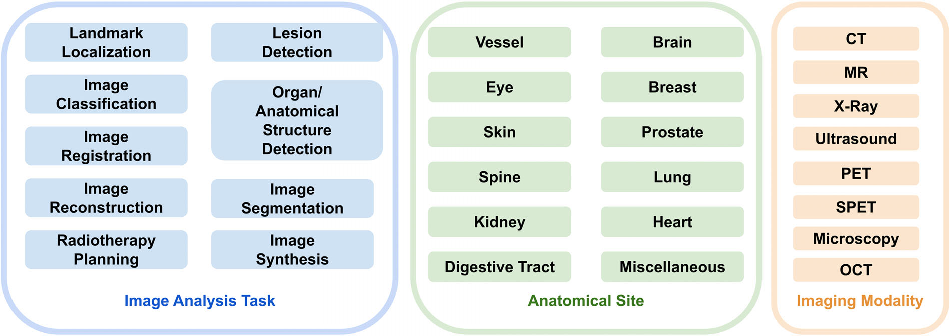
\includegraphics[width=0.98\linewidth]{images/Blue.pdf}
    \caption{Blue box covers image analysis tasks; green box covers anatomical sites; yellow box covers imaging modalities.}
    \label{fig:applications_of_rl_in_medical_imaging}
\end{figure*}


Importantly, RL offers several key mechanisms to alleviate data scarcity in medical imaging:

\begin{itemize}
    \item \textbf{Minimal dependence on annotations:} RL agents can learn optimal behaviors by interacting with environments, reducing reliance on large-scale annotated datasets.
    \item \textbf{Higher sample efficiency:} Especially in model-based RL, agents require fewer interactions to achieve comparable performance, making them well-suited for small datasets.
    \item \textbf{Active data selection:} RL-based frameworks have been proposed to select the most informative samples for annotation or training, optimizing the use of limited labeled data.
    \item \textbf{Combination with generative models:} RL can be integrated with GANs or VAEs to select high-quality synthetic samples for augmentation, effectively enhancing dataset diversity.
\end{itemize}

Overall, reinforcement learning not only reduces the burden of manual annotation but also promotes the development of data-efficient, adaptive, and goal-driven medical image analysis systems. Its ability to model complex sequential decision-making makes it a promising tool for next-generation clinical AI.



\subsection{Generative Models for Medical Image Synthesis}
The scarcity of large, diverse, and annotated medical imaging datasets remains a significant bottleneck in developing robust AI models for clinical applications. Generative models, particularly ​​Generative Adversarial Networks (GANs)\cite{Goodfellow2014GenerativeAN}​​ and ​​diffusion models​\cite{SohlDickstein2015DeepUL}​, have emerged as powerful tools to mitigate this challenge by synthesizing high-fidelity medical images that augment limited real-world datasets \cite{koetzierGeneratingSyntheticData2024}. These models learn the underlying data distribution of training images and generate novel samples that preserve anatomical and pathological features while ensuring patient privacy.

\subsubsection{Generative Adversarial Networks (GANs)}
GANs consist of a ​​generator​​ (creates synthetic images) and a ​​discriminator​​ (distinguishes real from synthetic images). Through adversarial training, the generator improves realism\cite{Goodfellow2014GenerativeAN}.

For example, Upadhyay et al. (2024)\cite{wangGenerationSyntheticGround2022} proposed a GAN-based framework to generate synthetic lung lesions mimicking ground glass nodules (GGNs), addressing the data scarcity issue in computer-aided diagnosis systems. The model consists of a generator and a discriminator trained adversarially to produce realistic synthetic GGNs.

The generator employs a U-Net-like architecture to synthesize GGNs\cite{8099502}, while the discriminator uses convolutional layers\cite{He2015DeepRL} to distinguish real from synthetic images. The loss function combines adversarial loss with pixel-wise reconstruction loss to ensure both realism and anatomical accuracy.

The model consists of three key components:
\begin{itemize}
\item \textbf{Generator (G)}: SRGAN-based network that synthesizes pulmonary nodules from masked input images
\item \textbf{ROI Discriminator ($D_{ROI}$)}: ResNet-based classifier operating on nodule regions (red path in Fig.\ref{fig:gan_architecture})
\item \textbf{Whole Image Discriminator ($D_{whole}$)}: Parallel ResNet evaluating full contextual realism (blue path)
\end{itemize}

\begin{figure*}[htb]
    \centering
    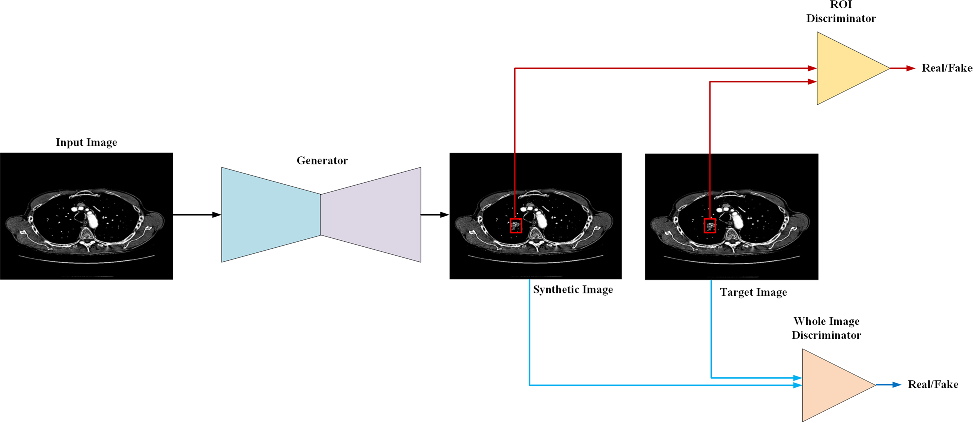
\includegraphics[width=0.98\linewidth]{images/GAN_model.pdf}
    \caption{A schematic overview of a diffusion model in training and sampling settings. In the top row, the diffusion model is trained and creates a Markov chain to add Gaussian noise to the real images, resulting in a noise vector z’. The model then reverses the Markov chain by predicting the next state of the image from the current noisy state, which is equivalent to denoising the image. During sampling (bottom row), the model can generate synthetic images by starting from a random noise vector and applying the reverse Markov chain.}
    \label{fig:gan_architecture}
\end{figure*}

The composite loss combines adversarial and similarity terms for both discriminators:

\begin{align}
\mathcal{L}_{DSRGAN} &= (\mathcal{L}_{sim} + \mathcal{L}_{adv})_{whole} + (\mathcal{L}_{sim} + \mathcal{L}_{adv})_{ROI} \\
\mathcal{L}_{adv} &= \sum_{n=1}^N -\log D(G(x)) \\
\mathcal{L}_{sim}(x,y) &= 1 - \frac{(2\mu_x\mu_y + C_1) + (\sigma_{xy} + C_2)}{(\mu_x^2 + \mu_y^2 + C_1)(\sigma_x^2 + \sigma_y^2 + C_2)}
\end{align}

where $\mu,\sigma$ denote mean/variance of image patches, $C_1,C_2$ stabilize division.

% \begin{algorithm}[htb
%     ]
%     \caption{Dual-Discriminator GAN Training}
%     \label{alg:ddgan}
%     \begin{algorithmic}[1]
%     \STATE Initialize generator $G$, ROI discriminator $D_{\text{ROI}}$, and whole image discriminator $D_{\text{whole}}$ with pre-trained SRGAN/ResNet weights
%     \FOR{each training batch}
%         \STATE Load input image $x_{\text{in}}$ (with erased ROI) and ground truth $x_{\text{target}}$
%         \STATE Generate synthetic image: $\hat{x} \leftarrow G(x_{\text{in}})$
        
%         \STATE \textbf{Update $D_{\text{ROI}}$:}
%         \STATE Extract ROI patches: $p_{\text{real}} \leftarrow x_{\text{target}}$, $p_{\text{fake}} \leftarrow \hat{x}$
%         \STATE Compute discriminator loss: 
%         \[
%             \mathcal{L}_{D_{\text{ROI}}} = -\log D_{\text{ROI}}(p_{\text{real}}) - \log\left(1 - D_{\text{ROI}}(p_{\text{fake}})\right)
%         \]
%         \STATE Update $D_{\text{ROI}}$ via gradient descent on $\nabla_{\theta_{D_{\text{ROI}}}} \mathcal{L}_{D_{\text{ROI}}}$
        
%         \STATE \textbf{Update $D_{\text{whole}}$:}
%         \STATE Compute loss:
%         \[
%             \mathcal{L}_{D_{\text{whole}}} = -\log D_{\text{whole}}(x_{\text{target}}) - \log\left(1 - D_{\text{whole}}(\hat{x})\right)
%         \]
%         \STATE Update $D_{\text{whole}}$ via gradient descent on $\nabla_{\theta_{D_{\text{whole}}}} \mathcal{L}_{D_{\text{whole}}}$
    
%         \STATE \textbf{Update Generator $G$:}
%         \STATE Compute adversarial loss:
%         \[
%             \mathcal{L}_{\text{adv}} = -\log D_{\text{ROI}}(\hat{x}) - \log D_{\text{whole}}(\hat{x})
%         \]
%         \STATE Compute similarity loss $\mathcal{L}_{\text{sim}}$ (see Eq.~3)
%         \STATE Update $G$ by minimizing:
%         \[
%             \nabla_{\theta_G} \left( \lambda_{\text{adv}} \mathcal{L}_{\text{adv}} + \lambda_{\text{sim}} \mathcal{L}_{\text{sim}} \right)
%         \]
%     \ENDFOR
%     \end{algorithmic}
% \end{algorithm}
    
The result of the GAN training is a generator capable of producing synthetic GGNs that closely resemble real lesions, as shown in Figure \ref{fig:gan_results}. The generated images can be used to augment existing datasets, improving the performance of downstream tasks such as classification and segmentation.

\begin{figure}[htb]
    \centering
    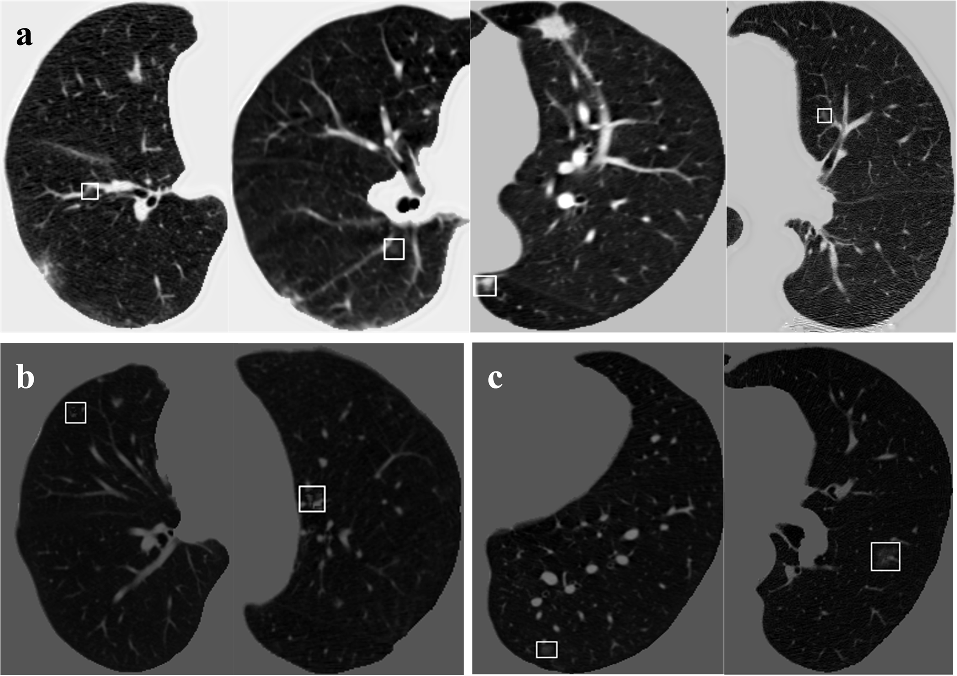
\includegraphics[width=0.98\linewidth]{images/gan_result.pdf}
    \caption{Examples of synthetic ground glass nodules (GGNs), the GGNs were categorised by physicians to four categories: confidently fake, leaning fake, leaning real, and confidently real. a Synthetic GGNs classified as “real” by clinicians. b Synthetic GGNs with less convincing generated lesions (classified as “leaning fake”). c A real GGNs in the original LIDC-IDRI dataset}
    \label{fig:gan_results}
\end{figure}

\subsubsection{Diffusion Models}
Diffusion models are a class of generative models that learn to generate data by reversing a diffusion process. They have gained popularity due to their ability to produce high-quality samples and have been successfully applied in various domains, including image synthesis, text generation, and audio processing\cite{songScoreBasedGenerativeModeling2021}.

Figure \ref{fig:diffusion_model_architecture} illustrates the training and sampling process of the diffusion model, showcasing how noise is added and subsequently removed to generate synthetic images.

\begin{figure*}[htb]
    \centering
    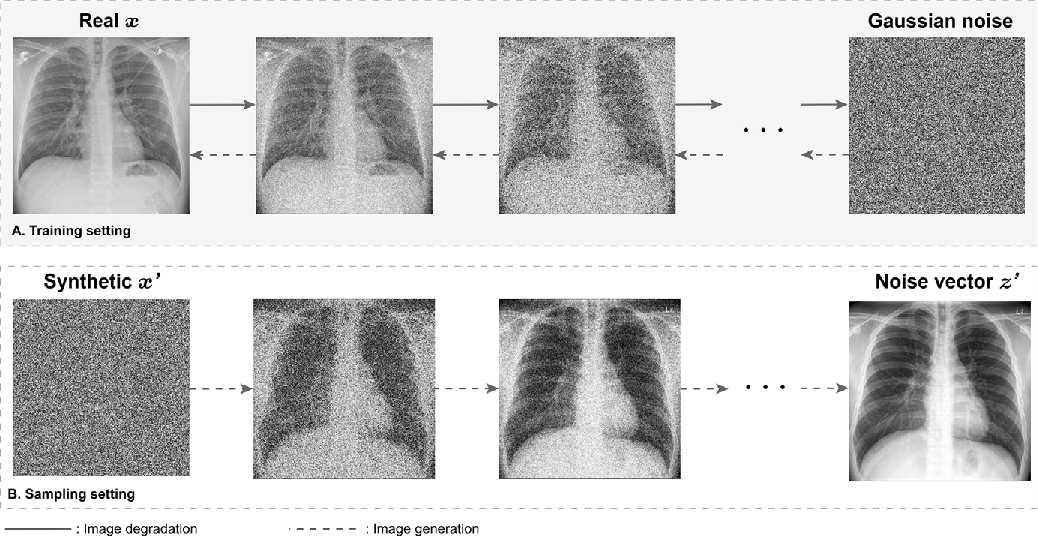
\includegraphics[width=0.98\linewidth]{images/diffusion_model.pdf}
    \caption{A schematic overview of a diffusion model in training and sampling settings. In the top row, the diffusion model is trained and creates a Markov chain to add Gaussian noise to the real images, resulting in a noise vector z’. The model then reverses the Markov chain by predicting the next state of the image from the current noisy state, which is equivalent to denoising the image. During sampling (bottom row), the model can generate synthetic images by starting from a random noise vector and applying the reverse Markov chain.}
    \label{fig:diffusion_model_architecture}
\end{figure*}

Consider a sequence of positive noise scales $0 < \beta_1, \dots, \beta_N < 1$. For each training data point $x_0 \sim p_{data}(x)$, construct a discrete Markov chain $\{X_0, X_1, \dots, X_N\}$ where:

\begin{equation}
p(x_t|x_{t-1}) = \mathcal{N}(x_t; \sqrt{1-\beta_t}x_{t-1}, \beta_t\mathbf{I})
\end{equation}

The marginal distribution after $t$ steps becomes:

\begin{equation}
q_t(x_t|x_0) = \mathcal{N}(x_t; \sqrt{\alpha_t}x_0, (1-\alpha_t)\mathbf{I}), \quad \alpha_t = \prod_{s=1}^t (1-\beta_s)
\end{equation}

The perturbed data distribution is defined as:

\begin{equation}
p_{\alpha_t}(\tilde{x}) = \int p_{data}(x)q_{\alpha_t}(\tilde{x}|x)dx
\end{equation}

with noise scales chosen such that $X_N \approx \mathcal{N}(0,\mathbf{I})$.

The variational Markov chain in the reverse direction is parameterized as:

\begin{equation}
p_\theta(x_{t-1}|x_t) = \mathcal{N}\left(x_{t-1}; \frac{1}{\sqrt{1-\beta_t}}(x_t + \beta_t s_\theta(x_t,t)), \beta_t\mathbf{I}\right)
\end{equation}

The model is trained with a re-weighted ELBO variant:

\begin{equation}
\theta^* = \arg\min_\theta \sum_{t=1}^N (1-\alpha_t) \mathbb{E}_{p_{data}(x)}\mathbb{E}_{q_t(\tilde{x}|x)} \| s_\theta(\tilde{x},t) - \nabla_x \log q_t(\tilde{x}|x) \|_2^2
\end{equation}

After obtaining the optimal model $s_\theta^*$, samples's generation is as shown in Algorithm \ref{alg:ddpm_sampling}. 

\begin{algorithm}[H]
\caption{DDPM Ancestral Sampling}
\label{alg:ddpm_sampling}
\begin{algorithmic}[1]
\STATE Initialize $x_N \sim \mathcal{N}(0,\mathbf{I})$
\FOR{$t = N$ downto $1$}
    \STATE $x_{t-1} = \frac{1}{\sqrt{1-\beta_t}}(x_t + \beta_t s_\theta^*(x_t,t)) + \sqrt{\beta_t}z_t$, $z_t \sim \mathcal{N}(0,\mathbf{I})$
\ENDFOR
\STATE Return $x_0$
\end{algorithmic}
\end{algorithm}

Diffusion models are particularly well-suited for medical image generation due to their ability to produce high-quality, diverse, and anatomically accurate synthetic images. Their iterative denoising process ensures fine-grained control over the generated data, preserving critical medical details. Additionally, diffusion models are robust to noise and can effectively model complex data distributions, making them ideal for handling the variability and precision required in medical imaging. These characteristics make diffusion models a powerful tool for augmenting datasets, improving model generalization, and addressing data scarcity challenges in medical imaging applications.



    







\section{Ethical Considerations in Applying AI to Medical Imaging}
\label{sec:ethical_implications}
The integration of AI into medical imaging has yielded impressive results, but also raises several ethical concerns. These issues must be thoroughly addressed to ensure safe, equitable, and trustworthy deployment of AI systems in healthcare.


\subsection{Data Privacy and Security}
The collection and use of medical imaging data raise significant privacy concerns due to the personal nature of health information. Patient data is strictly protected by various regulations such as HIPAA in the United States, GDPR in Europe, and similar frameworks globally. These regulations impose strict requirements on data sharing and access, which can significantly impede the development of robust AI models \cite{koetzierGeneratingSyntheticData2024}.

Synthetic data generation techniques, as discussed in Section \ref{sec:ml_technologies}, offer a promising solution to these privacy challenges. By creating artificial medical images that preserve the statistical properties and clinical relevance of real images without containing actual patient information, these approaches can effectively circumvent many privacy concerns:

\begin{itemize}
    \item \textbf{Risk Mitigation}: Synthetic data eliminates the risk of exposing protected health information (PHI), as the generated images do not correspond to real patients. This significantly reduces the regulatory burden and potential legal liability associated with data breaches.
    
    \item \textbf{Enhanced Data Sharing}: Synthetic datasets can be more freely shared across institutions and international boundaries, facilitating collaborative research and development without privacy impediments.
    
    \item \textbf{Data Augmentation}: As demonstrated in our GAN and diffusion model implementations, synthetic images can augment limited real datasets, addressing both privacy concerns and data scarcity simultaneously.
\end{itemize}

However, synthetic data is not without its own security considerations. Particularly, models like GANs might inadvertently memorize training examples, potentially leading to data leakage if not properly safeguarded. Additionally, adversarial attacks on these generative models could potentially extract sensitive information from the training data. Rigorous security measures, including proper model evaluation for memorization, differential privacy techniques during training, and robust access controls, must be implemented to ensure synthetic data approaches maintain strong privacy guarantees \cite{koetzierGeneratingSyntheticData2024}.

The self-supervised learning approaches described earlier provide another privacy-preserving advantage: they can extract valuable information from unlabeled data without requiring detailed annotations that might contain sensitive information. By learning from the inherent structure of images rather than explicit labels, techniques like context restoration minimize exposure to privacy-sensitive metadata.

\subsection{Bias and Fairness}
AI systems for medical imaging are inherently shaped by the data used to train them, making them susceptible to perpetuating or even amplifying existing biases in healthcare. This is particularly concerning in the context of data scarcity, where models might be developed using imbalanced or non-representative datasets \cite{koetzierGeneratingSyntheticData2024}.

Several types of bias can manifest in medical imaging AI:

\begin{itemize}
    \item \textbf{Demographic Bias}: When training data lacks diversity across age, gender, ethnicity, or socioeconomic factors, resulting models may perform disproportionately poorly on underrepresented groups. For example, models trained predominantly on data from certain ethnic populations may show reduced accuracy when applied to different demographic groups.
    
    \item \textbf{Technical Bias}: Variations in imaging equipment, acquisition protocols, and institutional practices introduce substantial heterogeneity in medical images. Models trained on data from high-end scanners may perform poorly on images from lower-resource settings, potentially exacerbating healthcare disparities.
    
    \item \textbf{Selection Bias}: The process of collecting training data often introduces sampling biases. For instance, data from academic medical centers may overrepresent rare or complex cases compared to community hospitals.
\end{itemize}

The generative approaches discussed in Section \ref{sec:ml_technologies}, while addressing data scarcity, introduce their own fairness considerations. GANs and diffusion models tend to capture and potentially amplify patterns present in their training data. If the training data contains biases, synthetic data generated from these models may inherently encode and propagate these biases, potentially worsening the problem rather than solving it.

To mitigate these risks, synthetic data generation should be specifically designed with fairness in mind:

\begin{itemize}
    \item \textbf{Balanced Data Generation}: Generative models can be explicitly conditioned to produce balanced distributions across demographic factors or modalities, potentially oversampling underrepresented groups.
    
    \item \textbf{Fairness-Aware Training}: Incorporating fairness constraints or adversarial debiasing techniques into generative model training can help reduce the transfer of biases to synthetic data.
    
    \item \textbf{Diverse Data Sources}: Incorporating data from diverse sites and populations, even if in small quantities, can help generative models capture broader variations in anatomical structures and pathologies.
\end{itemize}


\subsection{Transparency and Explainability}
The "black-box" nature of many advanced AI systems used in medical imaging poses significant challenges for clinical adoption and regulatory approval. Complex models like deep generative networks and self-supervised learning approaches often lack transparency in their decision-making processes, making it difficult for healthcare professionals to understand and trust their outputs\cite{vermaRoleDeepLearning2023}.

In medical contexts, where decisions directly impact patient outcomes, this lack of explainability is particularly problematic:

\begin{itemize}
    \item \textbf{End-to-end Generative Models}: GANs and diffusion models operate as black boxes, taking inputs and producing synthetic images through complex transformations that are not easily interpretable. The multi-layer, non-linear nature of these models makes it virtually impossible to trace exactly how specific features in the generated images were constructed.
    
    \item \textbf{Self-Supervised Learning}: While SSL methods effectively learn from unlabeled data, the representations they develop are often abstract and difficult to map to clinically meaningful features. The pretext tasks (like context restoration) may have little direct relationship to the downstream diagnostic tasks.
    
    \item \textbf{Reinforcement Learning}: Among the approaches discussed, RL may offer slightly better explainability through its explicit reward functions and state-action mappings, but complex neural network policies still suffer from opacity in their internal reasoning.
\end{itemize}

To address these challenges, several approaches are being developed to enhance the explainability of AI in medical imaging:

\begin{itemize}
    
    \item \textbf{Counterfactual Explanations}: Generating "what-if" scenarios that demonstrate how changes to the input would affect the output helps users understand the model's decision boundaries.
    
    \item \textbf{Layer-wise Relevance Propagation}: This technique decomposes predictions into contributions from individual input features, creating heatmaps that visualize important regions.
    
    \item \textbf{Feature Disentanglement}: Particularly for generative models, encouraging the separation of clinically relevant features (e.g., anatomical structures, pathologies) into interpretable latent dimensions improves transparency.
\end{itemize}


\subsection{Accountability and Governance}
In medical imaging, where AI impacts patient care, robust accountability and governance frameworks are critical. The discussed AI approaches—generative models, self-supervised learning, and reinforcement learning—pose unique challenges, especially in data-scarce contexts.

\begin{itemize}
    \item \textbf{Clinical Validation}: AI systems using limited or synthetic data must undergo rigorous testing across diverse populations with clear performance metrics and post-deployment monitoring.
    \item \textbf{Responsibility Assignment}: Clear accountability frameworks are needed to define responsibility for errors, especially with models trained on synthetic or limited data.
    \item \textbf{Regulatory Oversight}: Evolving frameworks, like those from the FDA, must address challenges specific to data-scarce and generative AI systems.
\end{itemize}

Governance of synthetic data requires attention to:

\begin{itemize}
    \item \textbf{Quality Control}: Ensure synthetic images meet clinical standards and represent pathological features accurately.
    \item \textbf{Provenance Tracking}: Maintain records distinguishing real and synthetic data for transparency.
    \item \textbf{Continuous Evaluation}: Regularly reassess models trained on synthetic data to ensure reliability.
\end{itemize}

For self-supervised and reinforcement learning:

\begin{itemize}
    \item \textbf{Pretext Task Validation}: Ensure self-supervised tasks produce clinically relevant representations.
    \item \textbf{Reward Function Oversight}: Design RL reward functions collaboratively with clinicians to ensure meaningful outcomes.
    \item \textbf{Update Protocols}: Define clear guidelines for model updates and recertification.
\end{itemize}

Multidisciplinary committees and international standards are essential to ensure safety, efficacy, and equity in deploying AI in data-scarce medical domains.

\section{Conclusion}
\label{sec:conc}

This paper explored how artificial intelligence and machine learning technologies can address data scarcity challenges in medical imaging. We examined three key approaches: self-supervised learning, reinforcement learning, and generative models. Self-supervised learning effectively leverages unlabeled data through pretext tasks like context restoration. Reinforcement learning offers learning from limited feedback rather than extensive labeled datasets. Generative models, including GANs and diffusion models, synthesize realistic medical images to augment limited datasets while preserving patient privacy. 

While these technologies show great promise, ethical considerations around privacy, bias, transparency, and governance remain crucial. With continued research and responsible implementation, AI technologies can help overcome data limitations, potentially improving healthcare access and outcomes across diverse clinical settings.


\vfill\pagebreak

% References should be produced using the bibtex program from suitable
% BiBTeX files (here: strings, refs, manuals). The IEEEbib.bst bibliography
% style file from IEEE produces unsorted bibliography list.
% -------------------------------------------------------------------------
\bibliographystyle{IEEEbib}
\bibliography{refs}

\end{document}
